\documentclass{beamer}

\usepackage[utf8]{inputenc}
\usepackage{default}


\usepackage{multirow} %for aligning stuff in tables

\usepackage{bbding} %for the smiley face

\usepackage{calc} %calculate spacing \widthof

%tikz stuff
\usepackage{tikzsymbols}
\usepackage{tikz}
\usetikzlibrary{fit,arrows,positioning}

  % Keys to support piece-wise uncovering of elements in TikZ pictures:
  % \node[visible on=<2->](foo){Foo}
  % \node[visible on=<{2,4}>](bar){Bar}   % put braces around comma expressions
  %
  % Internally works by setting opacity=0 when invisible, which has the
  % adavantage (compared to \node<2->(foo){Foo} that the node is always there, hence
  % always consumes space plus that coordinate (foo) is always available.
  %
  % The actual command that implements the invisibility can be overriden
  % by altering the style invisible. For instance \tikzsset{invisible/.style={opacity=0.2}}
  % would dim the "invisible" parts. Alternatively, the color might be set to white, if the
  % output driver does not support transparencies (e.g., PS)
  %
  \tikzset{
    invisible/.style={opacity=0},
    visible on/.style={alt={#1{}{invisible}}},
    alt/.code args={<#1>#2#3}{%
      \alt<#1>{\pgfkeysalso{#2}}{\pgfkeysalso{#3}} % \pgfkeysalso doesn't change the path
    },
  }
  \tikzset{
    dimmed/.style={opacity=0.2},
    dimmed on/.style={alt={#1{dimmed}{}}},
    alt/.code args={<#1>#2#3}{%
      \alt<#1>{\pgfkeysalso{#2}}{\pgfkeysalso{#3}} % \pgfkeysalso doesn't change the path
    },
  }
\tikzset{
    %Define standard arrow tip
    >=stealth',
    %Define style for boxes
    peer/.style={
           rectangle,
           rounded corners,
           draw=black, thin,
           text width=3.5em,
           minimum height=2em,
           text centered},
    node/.style={
           rectangle,
           rounded corners,
           draw=black,
           text width=4.5em,
           minimum height=2em,
           text centered,
           fill={rgb:black,1;white,3}},
    chunk/.style={
           rectangle,
           rounded corners,
           draw=black,
           text width=2.5em,
           minimum height=1em,
           text centered,
           fill=block title bg},
    % Define arrow style
    point/.style={
           ->,
           thick,
           shorten <=2pt,
           shorten >=2pt,}
every node/.style={align=center}
}

\newcommand{\wholeslide}[2][]{
\begin{frame}{#1}
% \transboxout<1>[duration=0.5]
\setbeamercolor{bgcolor}{fg=black,bg=white}
\begin{tikzpicture}[overlay, remember picture]
\node[anchor=center] at (current page.center) {
  \begin{beamercolorbox}[center]{bgcolor}
     #2
  \end{beamercolorbox}};
\end{tikzpicture}

\end{frame}
}

\newcommand{\blankslide}[2][]{
\begin{frame}[plain]{#1}
% \transboxout<1>[duration=0.5]
\setbeamercolor{bgcolor}{fg=black,bg=white}
\begin{tikzpicture}[overlay, remember picture]
\node[anchor=center] at (current page.center) {
  \begin{beamercolorbox}[center]{bgcolor}
     #2
  \end{beamercolorbox}};
\end{tikzpicture}

\end{frame}
}

\newenvironment<>{varblock}[2][.9\textwidth]{%
  \setlength{\textwidth}{#1}
  \begin{actionenv}#3%
    \def\insertblocktitle{#2}%
    \par%
    \usebeamertemplate{block begin}}
  {\par%
    \usebeamertemplate{block end}%
  \end{actionenv}}

\newlength{\mywidth}
\newcommand{\blockslide}[3][]{
\settowidth{\mywidth}{#3}
\begin{frame}[c]{#1}
\begin{center}
\begin{minipage}{1.1\mywidth}
 \begin{varblock}[1.1\mywidth]{#2}
  #3
 \end{varblock}
\end{minipage}
\end{center}
\end{frame}
}


\newcommand{\plainblockslide}[2]{
\settowidth{\mywidth}{#2}
\begin{frame}[c]
\begin{center}
\begin{minipage}{1.1\mywidth}
 \begin{varblock}[1.1\mywidth]{#1}
  #2
 \end{varblock}
\end{minipage}
\end{center}
\end{frame}
}

\mode<presentation>{
\usetheme{Warsaw}\usecolortheme{crane}
\setbeamertemplate{items}[square]
\setbeamertemplate{section in toc}[square]
\setbeamertemplate{subsection in toc}[square]
% \setbeamertemplate{subsection in toc}[subsections numbered]
\setbeamertemplate{subsubsection in toc}[square]
% \setbeamercolor{items}{fg=black,bg=yellow}
\usebeamercolor{block title}
\definecolor{block title bg}{named}{bg}
\setbeamercolor{item projected}{fg=black,bg=block title bg}
\setbeamercolor{itemize item}{fg=block title bg,bg=block title bg}
}







\title{\textsc{swap, swear and swindle}: \\incentive system for swarm and beyond}
\author{Viktor Trón and Aron Fischer}

\AtBeginSection[]
{
\begin{frame}<beamer>
\frametitle{Outline}
\tableofcontents[currentsection,sectionstyle=show/shaded,subsectionstyle=show/show/shaded,subsubsectionstyle=show/show/show/hide]
\end{frame}
}

\begin{document}

\begin{frame}
 \titlepage
\end{frame}

\blankslide{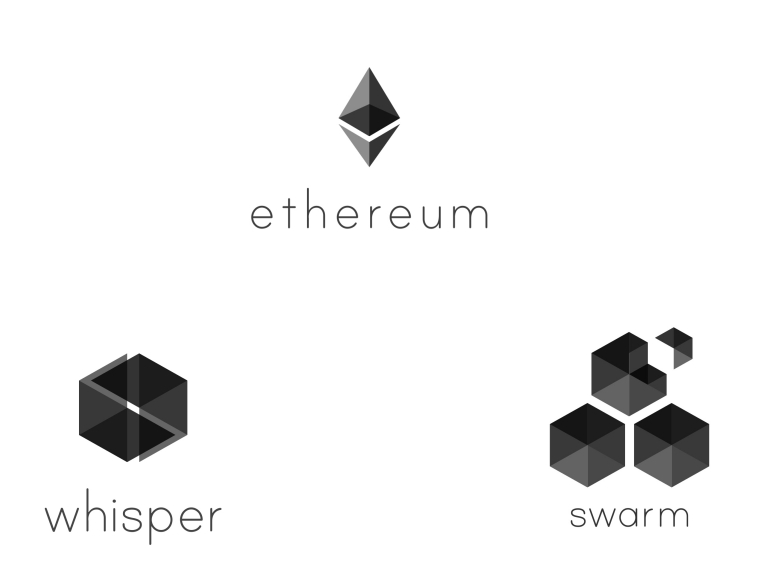
\includegraphics[width=0.8\textwidth]{ecosystem0.jpg}}

\begin{frame}{Outline}
 \tableofcontents[subsectionstyle=shaded/shaded,subsubsectionstyle=show/hide/hide]
\end{frame}

\begin{section}{content delivery}


\subsection{data retrieval}
\blockslide{\textbf{data out}}{How to retrieve data stored in the swarm.}


\begin{frame}{data retrieval}
\begin{columns}[T]
\begin{column}{0.4\textwidth}
\small
\begin{itemize}
\item<1-> node id, chunk id, function as addresses in the same keyspace
\item<4-> dapp retrieves \texttt{awesome-swarm-slides.pdf}
\item<5-> get its address \textbf{H}
\item<6-> content with address \textbf{H} stored with the node whose own address is \emph{closest} to \textbf{H}
\item<7-> swarm's \textbf{retrieval process} is responsible for deliviering
\end{itemize}
\end{column}

\begin{column}{0.6\textwidth}
\begin{tikzpicture}
 \node[scale=0.7]{
    \begin{tikzpicture}
      \node[visible on=<2->] at (2,2) {\textbf{the swarm network:}};

      \node[node,visible on=<2->] at (0,0) {};
      \node[node,visible on=<2->] at (1,-0.9) {};
      \node[node,visible on=<2->] at (0.5,-3) {};
      \node[node,visible on=<2->] at (0,-6.3) {};
      \node[node,visible on=<2->] at (5.8,-1.2) {};
      \node[node,visible on=<2->] at (4,-5.9) {};
      \node[node,visible on=<2->] at (4.1,-3) {};
      \node[node,visible on=<2->] at (2.1,-2) {};

      \node[node,visible on=<2>] at (4,0) (younode) {swarm-node};
      \node[peer,visible on=<3->] at (4,0) (you) {You};

      \node[visible on=<5->] (chunk) at (1,-5) {$\bullet$};
      \node[visible on=<5->] (chunklabel) at (2,-4.5) {H} edge[point,->,visible on =<5->] (chunk);

      \node[visible on=<2-6>, node] at (-0.5,-4.2) (close) {};
      \node[visible on=<7->, peer] at (-0.5,-4.2) (closestnode) {Closest Node};
      \node[visible on=<7->] at (-0.5, -5.5) (hlabel) {Look for ``H'' here}
    edge[visible on=<7->,point,->] (closestnode);
    \end{tikzpicture}
    };
\end{tikzpicture}
\end{column}
\end{columns}

\end{frame}






\begin{frame}{swarm retrieval process}

\begin{tikzpicture}
\node[peer,visible on=<1->] at (12,0) (retriever){retriever};
\node[visible on=<13>,scale=2] at (12,-1.5) {\Smiley};

\node[visible on=<2->] (chunk) at (4,-5) {$\bullet$};
\node[visible on=<2->] (chunklabel) at (3,-4) {data address} edge[point,->,visible on =<2->] (chunk);

\node[peer,visible on=<4-12>, dimmed on=<13->] at (8.5,-0.5) (connectedpeer){peer}
    (retriever.-150) edge[point, ->,visible on=<5>,dimmed on=<6-12>,  bend left=15]
      node[below=2pt,visible on=<5>, dimmed on=<6-12>] {request}
        (connectedpeer.-10);

\node[node,visible on=<6-11>, dimmed on=<12->] at (6,-2) (firstnode){some node}
  (connectedpeer.-70) edge[point,->,visible on=<6>, dimmed on=<7-11>,bend left=30]
      node[right of=2pt,visible on=<6>, dimmed on=<7-11>] {request}
        (firstnode.east);

\node[node,visible on=<7-10>, dimmed on=<11->] at (7.5,-4.5) (secondnode){other node}
  (firstnode.-70) edge[point,->,dashed,visible on=<7>, dimmed on=<8-10>,bend left=10]
      node[right of=2pt,visible on=<7>, dimmed on=<8-10>] {requests...}
        (secondnode.120);

\node[peer,visible on=<3-9>, dimmed on=<10->] at (4,-6) (closestnode){closest node}
  (secondnode.-110) edge[point,->,visible on=<8>, dimmed on=<9>,out=-110,in=0]
      node[right of=2pt,visible on=<8>, dimmed on=<9>] {request}
        (closestnode.east)
  (closestnode) edge[thick,point,->,visible on=<9>] node[above=2pt,visible on=<9>]{deliver} (secondnode)
  (secondnode.north west) edge[thick, point,->,visible on=<10>, dashed] node[left of=2pt,visible on=<10>]{deliveries} (firstnode.-120)
  (firstnode.55) edge[thick,point,->,visible on=<11>] node[left of=2pt,visible on=<11>]{deliver} (connectedpeer.-150)
  (connectedpeer) edge[thick,point,->,visible on=<12>] node[above=2pt,visible on=<12>]{deliver} (retriever)
  ;

\node[chunk, scale=0.6,visible on=<3->, below=3pt of closestnode.-50] {};
\node[chunk, scale=0.6,visible on=<9->, below=3pt of secondnode.-50] {};
\node[chunk, scale=0.6,visible on=<10->, below=3pt of firstnode.-50] {};
\node[chunk, scale=0.6,visible on=<11->, below=3pt of connectedpeer.-50] {};
\node[chunk, scale=0.6,visible on=<12->, below=3pt of retriever.-50] {};
\end{tikzpicture}
\end{frame}




\subsection[swap]{paying for data}
\plainblockslide{}{\textsc{swap}: \textbf{sw}arm \textbf{a}ccounting \textbf{p}rotocol}

\begin{frame}{\textsc{swap}: swarm accounting protocol}
\begin{columns}[T]
\begin{column}{0.5\textwidth}
\uncover<2->{\begin{block}{per-peer bandwidth accounting}
keeps track of all data retrieved both directions
\end{block}
}
\uncover<9->{
\begin{block}{settlement}
service for service or
tally too imbalanced $\rightarrow$ a \emph{payment} is initiated
\end{block}
}
\end{column}

\begin{column}{0.5\textwidth}
 \begin{center}
  \begin{tikzpicture}
   \node[peer,visible on=<3->] at (-2,0) (node1) {me};
   \node[peer,visible on=<4->] at (2,0) (node2) {peer}
   (node1.50) edge[point,->,dashed,visible on=<5->,bend right=30,out=50,in=130] node[below=10pt,visible on=<7->,scale=0.8] (sup){data delivered} (node2.130)
   (node2.-130) edge[point,->,dashed,visible on=<6->,bend left=30,in=130,out=50] node[above=10pt,visible on=<9->,scale=0.8]{data received} (node1.-50)
   ;
   \node[visible on=<8->,below= 2mm of sup]{\Large{-}};
  \end{tikzpicture}
 \end{center}
\end{column}

\end{columns}
\end{frame}

\begin{frame}{chequebook vs payment channel}
 \begin{itemize}
  \item \emph{not feasible} to pay for every chunk of data delivered with a transation
  \item<2-> even batch payments would constitute unacceptable blockchain bloat (and transaction cost).
 \end{itemize}
 \uncover<3->{instead of processing every payment on-chain, SWAP employs a \emph{chequebook} smart contract:}
  \begin{itemize}
  \item<4-> cheques are passed between connected swarm nodes (peers) off-chain.
  \item<4-> peers can cash in (process on-chain) the received cheques at any time.
  \item<4-> issued cheques are \emph{cumulative}, i.e., \textbf{only the last cheque needs to be cashed for settlement}.
 \end{itemize}
 \uncover<5>{\textsc{swap} will soon also be usable via \emph{payment channels} (see Raiden).}
\end{frame}

\begin{frame}{chequebook vs payment channel}
\begin{overlayarea}{\textwidth}{5.2cm}
\setbeamercovered{transparent}% Dim out "inactive" elements
\begin{columns}[t]
  \column{0.5\textwidth}
    \begin{block}{chequebook}
      \textbf{pro:}
      \begin{itemize}
       \item<1>{offchain payments}
       \item<2>{low barrier to entry (pay anyone)}
      \end{itemize}
      \textbf{con:}
      \begin{itemize}
       \item<3>{cheques can bounce (payment not guaranteed)}
      \end{itemize}
    \end{block}
  \column{0.5\textwidth}
    \begin{block}{channel}
      \textbf{pro:}
      \begin{itemize}
       \item<1>{offchain payments}
       \item<3>{secure - payments guaranteed}
      \end{itemize}
      \textbf{con:}
      \begin{itemize}
       \item<2>{high barrier to entry (must first join channel network)}
      \end{itemize}
    \end{block}
\end{columns}
\end{overlayarea}

\end{frame}

\begin{frame}
\begin{block}{SWARM + SWAP demonstrates}
\begin{itemize}
\item programmable incentives
\item drive towards low latency retrieval
\item auto-scaling delivery network
\end{itemize}
\end{block}
\end{frame}


\begin{frame}{swarm CDN is auto-scaling}
\begin{tikzpicture}
\node[peer,visible on=<1->] at (12,0) (retriever){};

\node[visible on=<1->] (chunk) at (4,-5) {$\bullet$};
\node[visible on=<1->] (chunklabel) at (3,-4) {data address} edge[point,->,visible on =<1->] (chunk);

\node[node,visible on=<2->,] at (8.5,-0.5) (connectedpeer){}
    (retriever.-150) edge[point, ->,visible on=<4-8>,  bend left=15]
      node[below=2pt,visible on=<4>] {request}
        (connectedpeer.-10);

\node[node,visible on=<2->] at (6,-2) (firstnode){}
  (connectedpeer.-70) edge[point,->,visible on=<4-7>,bend left=30]
      node[right of=2pt,visible on=<4>] {request}
        (firstnode.east);

\node[node,visible on=<2->] at (7.5,-4.5) (secondnode){}
  (firstnode.-70) edge[point,->,dashed,visible on=<4-6>,bend left=10]
      node[right of=2pt,visible on=<4>] {requests...}
        (secondnode.120);

\node[peer,visible on=<2->] at (4,-6) (closestnode){}
  (secondnode.-110) edge[point,->,visible on=<4-5>,out=-110,in=0]
      node[right of=2pt,visible on=<4>] {request}
        (closestnode.east)
  (closestnode) edge[thick,point,->,visible on=<5>] (secondnode)
  (secondnode.north west) edge[thick, point,->,visible on=<6>, dashed] (firstnode.-120)
  (firstnode.55) edge[thick,point,->,visible on=<7>] (connectedpeer.-150)
  (connectedpeer) edge[thick,point,->,visible on=<8>] (retriever)
  ;

\node[chunk, scale=0.6,visible on=<3->, below=3pt of closestnode.-50] {};
\node[chunk, scale=0.6,visible on=<5->, below=3pt of secondnode.-50] {};
\node[chunk, scale=0.6,visible on=<6-9>, below=3pt of firstnode.-50] {};
\node[chunk, scale=0.6,visible on=<7-9>, below=3pt of connectedpeer.-50] {};
\node[chunk, scale=0.6,visible on=<8->, below=3pt of retriever.-50] {};


\node[peer, visible on=<11->] at (12,-6) (newguy){};
\node[node, visible on=<11->] at (11,-4) (newnode){}
    (newguy) edge[point,->,visible on=<12-15>,dashed,bend left=20] (newnode)
    (newnode) edge[point,->,visible on=<13-14>,bend left=20] (secondnode)
    ;

\node[chunk, scale=0.6,visible on=<14->, below=3pt of newnode.-50] {}
    (secondnode) edge[thick,point,->,visible on=<14>] (newnode);
\node[chunk, scale=0.6,visible on=<15->, below=3pt of newguy.-50] {}
    (newnode) edge[thick,point,->,visible on=<15>] (newguy);

\node[visible on=<16>,scale=4] at (3,-1) {\Smiley};

\end{tikzpicture}
\end{frame}


\end{section}

\begin{section}{content storage}
\subsection[pay-as-you-store]{deferred payments and proof-of-custody}
\begin{frame}{}
SWAP allows for speedy retrieval of \emph{popular content}, but there is \textbf{no guarantee that less popular content will remain available}. Whatever is not accessed for a long time is likely to be deleted.\\[5mm]
The first step: change the swarm's incentives by \textbf{paying nodes to store your content}.
\end{frame}
\begin{frame}{payment for proof-of-custody}
The basic idea:
\begin{enumerate}
 \item commit in advance to paying for data to be available in the swarm.
 \item over time, challenge the swarm to provide proof that the data is still available: request \emph{proof-of-custody}.
 \item every valid proof-of-custody releases the next payment installment to the storing nodes.
\end{enumerate}
\begin{block}{Remember:}
 The \textbf{proof-of-custody} here is a small message - a single hash - which cryptographically proves that the issuer has access to the data.
\end{block}
\end{frame}
\begin{frame}{proof of custody + payment channel}
 These deferred payments  constitute a \textbf{conditional escrow}: payment is made up-front, payment is held (escrow) and is only released when a valid proof-of-custody is received (condition).\\[5mm]
 This procedure can be handled off-chain and can be directly \textbf{integrated into the payment channels.} All you need is a payment-channel \emph{judge contract} that can understand swarm storage receipts.
\end{frame}


\subsection[insurance]{storage insurance and negative incentives}
\begin{frame}{If data goes missing...}
 If data goes missing nodes will lose potential revenue for no longer being able to generate proofs-of-custody, but there are \emph{no further consequences} (yet). \\[5mm]
 Therefore, to complete the storage incentive scheme, we introduce an \emph{insurance system} the can \textbf{punish offending nodes for not keeping their storage promises}.
\end{frame}

\plainblockslide{}{\textsc{swear}: \textbf{sw}arm \textbf{e}nforcement of \textbf{a}rchiving \textbf{r}ules}


\begin{frame}{\textsc{swear} to store}
 SWEAR is a smart contract that allows nodes to register as long-term storage nodes by posting a \textbf{security deposit}.\\[5mm]
 Registered nodes can sell promissory notes guaranteeing long-term data availablilty -- essentially insurance against deleting. \\[5mm]
 Implementation: swarm syncing process with added receipts.
\end{frame}

\begin{frame}{the syncing process}
\begin{columns}[T]
\begin{column}{0.4\textwidth}
\only<1-10>{
\begin{block}{syncing}
  \begin{itemize}
  \item<3-> chunks to be stored at the nodes whose address is closest to the chunk ID
  \item<5-> relaying: syncing
  \item<7-> data is passed on from node to node
  % \item<10->[] %dummy. I needed this to get line spacing to work in the point above.
  \end{itemize}
\end{block}
}
\uncover<11>{\frametitle{insured upload to swarm}}
\only<11->{
\begin{block}{insured storage} syncing via registered nodes with each swap receipted.
\end{block}
\begin{block}{insured storage:}
\begin{itemize}
 \item owner passes data to a registered peer and receives an insurance receipt
 \item relaying: syncing
 \item all receipts are accounted and paid for
\end{itemize}
\end{block}
}
\end{column}

\begin{column}{0.6\textwidth}
\begin{tikzpicture}
 \node[scale=0.7,visible on=<1-10>] at (0,0) {
    \begin{tikzpicture}
  \node[invisible] at (0,-9) (dummy){};
  \node[invisible] at (5,-5) (dummy2){};
  \node[peer,visible on=<2->] at (-2,0) (owner){owner};

  \node[visible on=<3->] (chunk) at (4,-5) {$\bullet$};
  \node[visible on=<3->] (chunklabel) at (5,-4) {chunk address} edge[point,->,visible on =<3->] (chunk);

  \node[peer,visible on=<5->] at (0.5,-0.5) (connectedpeer){peer}
      (owner.east) edge[point, ->,visible on=<6->, bend left=15]
        node[above=2pt,visible on=<6->] {sync}
          (connectedpeer.150);

  \node[node,visible on=<7->] at (1,-2) (firstnode){some node}
    (connectedpeer.-70) edge[point,->,visible on=<7->,bend left=10]
        node[right of=2pt,visible on=<7->] {sync}
          (firstnode.north);

  \node[node,visible on=<8->] at (0.5,-4.5) (secondnode){other node}
    (firstnode.-70) edge[point,->,dashed,visible on=<8->,bend left=10]
        node[right of=2pt,visible on=<8->] {syncing...}
          (secondnode.70);

  \node[peer,visible on=<4->] at (4,-6) (closestnode){closest node}
    (secondnode.-110) edge[point,->,visible on=<9->,out=-110,in=180]
        node[above=2pt,visible on=<9->] {sync}
          (closestnode.west);
    \end{tikzpicture}
    };
 \node[scale=0.7,visible on=<12->] at (0,0) {
    \begin{tikzpicture}
  \node[invisible] at (0,-9) (dummy){};
  \node[invisible] at (5,-5) (dummy2){};
  \node[peer,visible on=<11->] at (-2,0) (owner){owner};

  \node[visible on=<12->] (chunk) at (4,-5) {$\bullet$};
  \node[visible on=<12->] (chunklabel) at (5,-4) {chunk address} edge[point,->,visible on =<11->] (chunk);

  \node[peer,visible on=<12->] at (0.5,-0.5) (connectedpeer){peer}
      (owner.east) edge[point, ->,visible on=<12->, bend left=15]
        node[above=2pt,visible on=<12->] {store}
          (connectedpeer.150)
      (connectedpeer.-170) edge[point,->,visible on=<12->,thick,bend right=15]  (owner.-20);

  \node[node,visible on=<12->] at (1,-2) (firstnode){some node}
    (connectedpeer.-70) edge[point,->,visible on=<12->,bend left=10]
        node[right of=2pt,visible on=<12->] {store}
          (firstnode.north)
      (firstnode.140) edge[point,->,visible on=<12->,thick,bend right=10] node[left of=2pt,visible on=<12->] {receipts} (connectedpeer.-140);

  \node[node,visible on=<12->] at (0.5,-4.5) (secondnode){other node}
    (firstnode.-70) edge[point,->,dashed,visible on=<12->,bend left=10]
        node[right of=2pt,visible on=<12->] {store...}
          (secondnode.70)
      (secondnode.110) edge[point,->,visible on=<12->,dashed,thick,bend right=10] node[left of=2pt,visible on=<12->] {receipts} (firstnode.-110);

  \node[peer,visible on=<12->] at (4,-6) (closestnode){closest node}
    (secondnode.-110) edge[point,->,visible on=<12->,out=-110,in=180]
        node[above=2pt,visible on=<12->] {store}
          (closestnode.west)
      (closestnode.-160) edge[point,->,visible on=<12->,thick,out=180,in=-110] node[left of=2pt,visible on=<12->] {receipt} (secondnode.-130);
    \end{tikzpicture}
    };
\end{tikzpicture}
\end{column}
\end{columns}
\end{frame}

\plainblockslide{}{\textsc{swindle}: \textbf{s}torage \textbf{w}ith \textbf{in}surance \textbf{d}eposit, \textbf{l}itigation and \textbf{e}scrow }
\blockslide[\textsc{swindle}]{TL;DR}{if insured data is lost, the storers lose their deposit}

\begin{frame}{litigation upon data loss}
\begin{block}{if insured data is not found}
%If insured data is lost, anyone holding a valid receipt can launch the litigation procedure.\\
%A node so challenged may defend itself by presenting
litigation by challenge
\end{block}
\begin{block}{defense by providing}
\begin{itemize}
 \item proof-of-custody of the data (eventually the data itself)
 \item a storage receipt for the data, shifting the blame and implicating another node as the culprit.
\end{itemize}
\end{block}
\begin{block}{upload and disappear}
\begin{itemize}
 \item swear to sync and receipting $\rightarrow$
immediate settlement with the peer at upload
 \item finger-pointing along chain of receipts $\rightarrow$
correct accountability of storer thereafter
\end{itemize}
\end{block}
%Only at the time of litigation is the chain from owner to storer explicitly determined.
%This is an important feature -- litigation may take time but initial storage can be fast allowing you to `upload and disappear'.
\end{frame}

\begin{frame}
 \begin{center}
 \textsc{ swap $\bullet$ swear $\bullet$ swindle }
 \end{center}
\end{frame}

\begin{frame}{ethersphere orange paper series}
 \begin{block}{}
Viktor Trón, Aron Fischer, Dániel Nagy A and Zsolt Felföldi, Nick Johnson: swap, swear and swindle: incentive system for swarm. May 2016
\end{block}
 \begin{block}{}
Viktor Trón, Aron Fischer, Nick Johnson: smash-proof: auditable storage for swarm secured by masked audit secret hash. May 2016
 \end{block}
\end{frame}

\end{section}

\begin{frame}{swarm: status and usage}
\begin{block}{what is the development status of swarm?}
\begin{enumerate}
\item golang implementation: proof-of-concept iteration 2 release 4, code has been merged to go-ethereum develop branch
\item Microsoft Azure hosting a testnet of 100+ nodes over 3 regions
\item expanding team, come join or contribute
\end{enumerate}
\end{block}

\begin{block}{how can swarm be used?}
\begin{itemize}
\item \texttt{bzzd} - swarm daemon, communicates with ethereum via IPC, so any ethereum client works
\item APIs: JSON RPC (via websockets, http, or ipc), http proxy, cli, fuse driver (planned)
\item API bindings: web3.js and CLI
\end{itemize}
\end{block}

\end{frame}


\begin{frame}[plain]{join us}

\begin{block}<1->{contact and contribute}

\begin{description}
\item[swarm channel:] \texttt{gitter.im/ethereum/swarm}
\item[swarm info page \& orange papers:] \texttt{swarm-gateways.net}
\item[swarm gateway:] \texttt{swarm-gateways.net} \texttt{web3.download}
\end{description}
\end{block}
\begin{block}{}
\begin{itemize}
\footnotesize
\item Daniel Nagy A., Nick Johnson, Viktor Trón, Zsolt Felföldi (core team)
\item Aron Fischer \& Ethersphere orange lounge group
\item Ram Devish, Bas van Kervel, Alex van der Sande (Mist integration)
\item Felix Lange (integration, devp2p)
\item Alex Beregszaszi (git, mango)
\item Igor Shadurin (file manager dapp)
\item Nick Johnson, Alex van der Sande (Ethereum Name Service)
\item Gavin Wood, Vitalik Buterin, Jeffrey Wilcke (visionaries)
\end{itemize}
\end{block}

\end{frame}



\end{document}
